\documentclass{article} % For LaTeX2e
\usepackage{iclr2022_conference,times}
% Optional math commands from https://github.com/goodfeli/dlbook_notation.
%%%%% NEW MATH DEFINITIONS %%%%%

\usepackage{amsmath,amsfonts,bm}

% Mark sections of captions for referring to divisions of figures
\newcommand{\figleft}{{\em (Left)}}
\newcommand{\figcenter}{{\em (Center)}}
\newcommand{\figright}{{\em (Right)}}
\newcommand{\figtop}{{\em (Top)}}
\newcommand{\figbottom}{{\em (Bottom)}}
\newcommand{\captiona}{{\em (a)}}
\newcommand{\captionb}{{\em (b)}}
\newcommand{\captionc}{{\em (c)}}
\newcommand{\captiond}{{\em (d)}}

% Highlight a newly defined term
\newcommand{\newterm}[1]{{\bf #1}}


% Figure reference, lower-case.
\def\figref#1{figure~\ref{#1}}
% Figure reference, capital. For start of sentence
\def\Figref#1{Figure~\ref{#1}}
\def\twofigref#1#2{figures \ref{#1} and \ref{#2}}
\def\quadfigref#1#2#3#4{figures \ref{#1}, \ref{#2}, \ref{#3} and \ref{#4}}
% Section reference, lower-case.
\def\secref#1{section~\ref{#1}}
% Section reference, capital.
\def\Secref#1{Section~\ref{#1}}
% Reference to two sections.
\def\twosecrefs#1#2{sections \ref{#1} and \ref{#2}}
% Reference to three sections.
\def\secrefs#1#2#3{sections \ref{#1}, \ref{#2} and \ref{#3}}
% Reference to an equation, lower-case.
\def\eqref#1{equation~\ref{#1}}
% Reference to an equation, upper case
\def\Eqref#1{Equation~\ref{#1}}
% A raw reference to an equation---avoid using if possible
\def\plaineqref#1{\ref{#1}}
% Reference to a chapter, lower-case.
\def\chapref#1{chapter~\ref{#1}}
% Reference to an equation, upper case.
\def\Chapref#1{Chapter~\ref{#1}}
% Reference to a range of chapters
\def\rangechapref#1#2{chapters\ref{#1}--\ref{#2}}
% Reference to an algorithm, lower-case.
\def\algref#1{algorithm~\ref{#1}}
% Reference to an algorithm, upper case.
\def\Algref#1{Algorithm~\ref{#1}}
\def\twoalgref#1#2{algorithms \ref{#1} and \ref{#2}}
\def\Twoalgref#1#2{Algorithms \ref{#1} and \ref{#2}}
% Reference to a part, lower case
\def\partref#1{part~\ref{#1}}
% Reference to a part, upper case
\def\Partref#1{Part~\ref{#1}}
\def\twopartref#1#2{parts \ref{#1} and \ref{#2}}

\def\ceil#1{\lceil #1 \rceil}
\def\floor#1{\lfloor #1 \rfloor}
\def\1{\bm{1}}
\newcommand{\train}{\mathcal{D}}
\newcommand{\valid}{\mathcal{D_{\mathrm{valid}}}}
\newcommand{\test}{\mathcal{D_{\mathrm{test}}}}

\def\eps{{\epsilon}}


% Random variables
\def\reta{{\textnormal{$\eta$}}}
\def\ra{{\textnormal{a}}}
\def\rb{{\textnormal{b}}}
\def\rc{{\textnormal{c}}}
\def\rd{{\textnormal{d}}}
\def\re{{\textnormal{e}}}
\def\rf{{\textnormal{f}}}
\def\rg{{\textnormal{g}}}
\def\rh{{\textnormal{h}}}
\def\ri{{\textnormal{i}}}
\def\rj{{\textnormal{j}}}
\def\rk{{\textnormal{k}}}
\def\rl{{\textnormal{l}}}
% rm is already a command, just don't name any random variables m
\def\rn{{\textnormal{n}}}
\def\ro{{\textnormal{o}}}
\def\rp{{\textnormal{p}}}
\def\rq{{\textnormal{q}}}
\def\rr{{\textnormal{r}}}
\def\rs{{\textnormal{s}}}
\def\rt{{\textnormal{t}}}
\def\ru{{\textnormal{u}}}
\def\rv{{\textnormal{v}}}
\def\rw{{\textnormal{w}}}
\def\rx{{\textnormal{x}}}
\def\ry{{\textnormal{y}}}
\def\rz{{\textnormal{z}}}

% Random vectors
\def\rvepsilon{{\mathbf{\epsilon}}}
\def\rvtheta{{\mathbf{\theta}}}
\def\rva{{\mathbf{a}}}
\def\rvb{{\mathbf{b}}}
\def\rvc{{\mathbf{c}}}
\def\rvd{{\mathbf{d}}}
\def\rve{{\mathbf{e}}}
\def\rvf{{\mathbf{f}}}
\def\rvg{{\mathbf{g}}}
\def\rvh{{\mathbf{h}}}
\def\rvu{{\mathbf{i}}}
\def\rvj{{\mathbf{j}}}
\def\rvk{{\mathbf{k}}}
\def\rvl{{\mathbf{l}}}
\def\rvm{{\mathbf{m}}}
\def\rvn{{\mathbf{n}}}
\def\rvo{{\mathbf{o}}}
\def\rvp{{\mathbf{p}}}
\def\rvq{{\mathbf{q}}}
\def\rvr{{\mathbf{r}}}
\def\rvs{{\mathbf{s}}}
\def\rvt{{\mathbf{t}}}
\def\rvu{{\mathbf{u}}}
\def\rvv{{\mathbf{v}}}
\def\rvw{{\mathbf{w}}}
\def\rvx{{\mathbf{x}}}
\def\rvy{{\mathbf{y}}}
\def\rvz{{\mathbf{z}}}

% Elements of random vectors
\def\erva{{\textnormal{a}}}
\def\ervb{{\textnormal{b}}}
\def\ervc{{\textnormal{c}}}
\def\ervd{{\textnormal{d}}}
\def\erve{{\textnormal{e}}}
\def\ervf{{\textnormal{f}}}
\def\ervg{{\textnormal{g}}}
\def\ervh{{\textnormal{h}}}
\def\ervi{{\textnormal{i}}}
\def\ervj{{\textnormal{j}}}
\def\ervk{{\textnormal{k}}}
\def\ervl{{\textnormal{l}}}
\def\ervm{{\textnormal{m}}}
\def\ervn{{\textnormal{n}}}
\def\ervo{{\textnormal{o}}}
\def\ervp{{\textnormal{p}}}
\def\ervq{{\textnormal{q}}}
\def\ervr{{\textnormal{r}}}
\def\ervs{{\textnormal{s}}}
\def\ervt{{\textnormal{t}}}
\def\ervu{{\textnormal{u}}}
\def\ervv{{\textnormal{v}}}
\def\ervw{{\textnormal{w}}}
\def\ervx{{\textnormal{x}}}
\def\ervy{{\textnormal{y}}}
\def\ervz{{\textnormal{z}}}

% Random matrices
\def\rmA{{\mathbf{A}}}
\def\rmB{{\mathbf{B}}}
\def\rmC{{\mathbf{C}}}
\def\rmD{{\mathbf{D}}}
\def\rmE{{\mathbf{E}}}
\def\rmF{{\mathbf{F}}}
\def\rmG{{\mathbf{G}}}
\def\rmH{{\mathbf{H}}}
\def\rmI{{\mathbf{I}}}
\def\rmJ{{\mathbf{J}}}
\def\rmK{{\mathbf{K}}}
\def\rmL{{\mathbf{L}}}
\def\rmM{{\mathbf{M}}}
\def\rmN{{\mathbf{N}}}
\def\rmO{{\mathbf{O}}}
\def\rmP{{\mathbf{P}}}
\def\rmQ{{\mathbf{Q}}}
\def\rmR{{\mathbf{R}}}
\def\rmS{{\mathbf{S}}}
\def\rmT{{\mathbf{T}}}
\def\rmU{{\mathbf{U}}}
\def\rmV{{\mathbf{V}}}
\def\rmW{{\mathbf{W}}}
\def\rmX{{\mathbf{X}}}
\def\rmY{{\mathbf{Y}}}
\def\rmZ{{\mathbf{Z}}}

% Elements of random matrices
\def\ermA{{\textnormal{A}}}
\def\ermB{{\textnormal{B}}}
\def\ermC{{\textnormal{C}}}
\def\ermD{{\textnormal{D}}}
\def\ermE{{\textnormal{E}}}
\def\ermF{{\textnormal{F}}}
\def\ermG{{\textnormal{G}}}
\def\ermH{{\textnormal{H}}}
\def\ermI{{\textnormal{I}}}
\def\ermJ{{\textnormal{J}}}
\def\ermK{{\textnormal{K}}}
\def\ermL{{\textnormal{L}}}
\def\ermM{{\textnormal{M}}}
\def\ermN{{\textnormal{N}}}
\def\ermO{{\textnormal{O}}}
\def\ermP{{\textnormal{P}}}
\def\ermQ{{\textnormal{Q}}}
\def\ermR{{\textnormal{R}}}
\def\ermS{{\textnormal{S}}}
\def\ermT{{\textnormal{T}}}
\def\ermU{{\textnormal{U}}}
\def\ermV{{\textnormal{V}}}
\def\ermW{{\textnormal{W}}}
\def\ermX{{\textnormal{X}}}
\def\ermY{{\textnormal{Y}}}
\def\ermZ{{\textnormal{Z}}}

% Vectors
\def\vzero{{\bm{0}}}
\def\vone{{\bm{1}}}
\def\vmu{{\bm{\mu}}}
\def\vtheta{{\bm{\theta}}}
\def\va{{\bm{a}}}
\def\vb{{\bm{b}}}
\def\vc{{\bm{c}}}
\def\vd{{\bm{d}}}
\def\ve{{\bm{e}}}
\def\vf{{\bm{f}}}
\def\vg{{\bm{g}}}
\def\vh{{\bm{h}}}
\def\vi{{\bm{i}}}
\def\vj{{\bm{j}}}
\def\vk{{\bm{k}}}
\def\vl{{\bm{l}}}
\def\vm{{\bm{m}}}
\def\vn{{\bm{n}}}
\def\vo{{\bm{o}}}
\def\vp{{\bm{p}}}
\def\vq{{\bm{q}}}
\def\vr{{\bm{r}}}
\def\vs{{\bm{s}}}
\def\vt{{\bm{t}}}
\def\vu{{\bm{u}}}
\def\vv{{\bm{v}}}
\def\vw{{\bm{w}}}
\def\vx{{\bm{x}}}
\def\vy{{\bm{y}}}
\def\vz{{\bm{z}}}

% Elements of vectors
\def\evalpha{{\alpha}}
\def\evbeta{{\beta}}
\def\evepsilon{{\epsilon}}
\def\evlambda{{\lambda}}
\def\evomega{{\omega}}
\def\evmu{{\mu}}
\def\evpsi{{\psi}}
\def\evsigma{{\sigma}}
\def\evtheta{{\theta}}
\def\eva{{a}}
\def\evb{{b}}
\def\evc{{c}}
\def\evd{{d}}
\def\eve{{e}}
\def\evf{{f}}
\def\evg{{g}}
\def\evh{{h}}
\def\evi{{i}}
\def\evj{{j}}
\def\evk{{k}}
\def\evl{{l}}
\def\evm{{m}}
\def\evn{{n}}
\def\evo{{o}}
\def\evp{{p}}
\def\evq{{q}}
\def\evr{{r}}
\def\evs{{s}}
\def\evt{{t}}
\def\evu{{u}}
\def\evv{{v}}
\def\evw{{w}}
\def\evx{{x}}
\def\evy{{y}}
\def\evz{{z}}

% Matrix
\def\mA{{\bm{A}}}
\def\mB{{\bm{B}}}
\def\mC{{\bm{C}}}
\def\mD{{\bm{D}}}
\def\mE{{\bm{E}}}
\def\mF{{\bm{F}}}
\def\mG{{\bm{G}}}
\def\mH{{\bm{H}}}
\def\mI{{\bm{I}}}
\def\mJ{{\bm{J}}}
\def\mK{{\bm{K}}}
\def\mL{{\bm{L}}}
\def\mM{{\bm{M}}}
\def\mN{{\bm{N}}}
\def\mO{{\bm{O}}}
\def\mP{{\bm{P}}}
\def\mQ{{\bm{Q}}}
\def\mR{{\bm{R}}}
\def\mS{{\bm{S}}}
\def\mT{{\bm{T}}}
\def\mU{{\bm{U}}}
\def\mV{{\bm{V}}}
\def\mW{{\bm{W}}}
\def\mX{{\bm{X}}}
\def\mY{{\bm{Y}}}
\def\mZ{{\bm{Z}}}
\def\mBeta{{\bm{\beta}}}
\def\mPhi{{\bm{\Phi}}}
\def\mLambda{{\bm{\Lambda}}}
\def\mSigma{{\bm{\Sigma}}}

% Tensor
\DeclareMathAlphabet{\mathsfit}{\encodingdefault}{\sfdefault}{m}{sl}
\SetMathAlphabet{\mathsfit}{bold}{\encodingdefault}{\sfdefault}{bx}{n}
\newcommand{\tens}[1]{\bm{\mathsfit{#1}}}
\def\tA{{\tens{A}}}
\def\tB{{\tens{B}}}
\def\tC{{\tens{C}}}
\def\tD{{\tens{D}}}
\def\tE{{\tens{E}}}
\def\tF{{\tens{F}}}
\def\tG{{\tens{G}}}
\def\tH{{\tens{H}}}
\def\tI{{\tens{I}}}
\def\tJ{{\tens{J}}}
\def\tK{{\tens{K}}}
\def\tL{{\tens{L}}}
\def\tM{{\tens{M}}}
\def\tN{{\tens{N}}}
\def\tO{{\tens{O}}}
\def\tP{{\tens{P}}}
\def\tQ{{\tens{Q}}}
\def\tR{{\tens{R}}}
\def\tS{{\tens{S}}}
\def\tT{{\tens{T}}}
\def\tU{{\tens{U}}}
\def\tV{{\tens{V}}}
\def\tW{{\tens{W}}}
\def\tX{{\tens{X}}}
\def\tY{{\tens{Y}}}
\def\tZ{{\tens{Z}}}


% Graph
\def\gA{{\mathcal{A}}}
\def\gB{{\mathcal{B}}}
\def\gC{{\mathcal{C}}}
\def\gD{{\mathcal{D}}}
\def\gE{{\mathcal{E}}}
\def\gF{{\mathcal{F}}}
\def\gG{{\mathcal{G}}}
\def\gH{{\mathcal{H}}}
\def\gI{{\mathcal{I}}}
\def\gJ{{\mathcal{J}}}
\def\gK{{\mathcal{K}}}
\def\gL{{\mathcal{L}}}
\def\gM{{\mathcal{M}}}
\def\gN{{\mathcal{N}}}
\def\gO{{\mathcal{O}}}
\def\gP{{\mathcal{P}}}
\def\gQ{{\mathcal{Q}}}
\def\gR{{\mathcal{R}}}
\def\gS{{\mathcal{S}}}
\def\gT{{\mathcal{T}}}
\def\gU{{\mathcal{U}}}
\def\gV{{\mathcal{V}}}
\def\gW{{\mathcal{W}}}
\def\gX{{\mathcal{X}}}
\def\gY{{\mathcal{Y}}}
\def\gZ{{\mathcal{Z}}}

% Sets
\def\sA{{\mathbb{A}}}
\def\sB{{\mathbb{B}}}
\def\sC{{\mathbb{C}}}
\def\sD{{\mathbb{D}}}
% Don't use a set called E, because this would be the same as our symbol
% for expectation.
\def\sF{{\mathbb{F}}}
\def\sG{{\mathbb{G}}}
\def\sH{{\mathbb{H}}}
\def\sI{{\mathbb{I}}}
\def\sJ{{\mathbb{J}}}
\def\sK{{\mathbb{K}}}
\def\sL{{\mathbb{L}}}
\def\sM{{\mathbb{M}}}
\def\sN{{\mathbb{N}}}
\def\sO{{\mathbb{O}}}
\def\sP{{\mathbb{P}}}
\def\sQ{{\mathbb{Q}}}
\def\sR{{\mathbb{R}}}
\def\sS{{\mathbb{S}}}
\def\sT{{\mathbb{T}}}
\def\sU{{\mathbb{U}}}
\def\sV{{\mathbb{V}}}
\def\sW{{\mathbb{W}}}
\def\sX{{\mathbb{X}}}
\def\sY{{\mathbb{Y}}}
\def\sZ{{\mathbb{Z}}}

% Entries of a matrix
\def\emLambda{{\Lambda}}
\def\emA{{A}}
\def\emB{{B}}
\def\emC{{C}}
\def\emD{{D}}
\def\emE{{E}}
\def\emF{{F}}
\def\emG{{G}}
\def\emH{{H}}
\def\emI{{I}}
\def\emJ{{J}}
\def\emK{{K}}
\def\emL{{L}}
\def\emM{{M}}
\def\emN{{N}}
\def\emO{{O}}
\def\emP{{P}}
\def\emQ{{Q}}
\def\emR{{R}}
\def\emS{{S}}
\def\emT{{T}}
\def\emU{{U}}
\def\emV{{V}}
\def\emW{{W}}
\def\emX{{X}}
\def\emY{{Y}}
\def\emZ{{Z}}
\def\emSigma{{\Sigma}}

% entries of a tensor
% Same font as tensor, without \bm wrapper
\newcommand{\etens}[1]{\mathsfit{#1}}
\def\etLambda{{\etens{\Lambda}}}
\def\etA{{\etens{A}}}
\def\etB{{\etens{B}}}
\def\etC{{\etens{C}}}
\def\etD{{\etens{D}}}
\def\etE{{\etens{E}}}
\def\etF{{\etens{F}}}
\def\etG{{\etens{G}}}
\def\etH{{\etens{H}}}
\def\etI{{\etens{I}}}
\def\etJ{{\etens{J}}}
\def\etK{{\etens{K}}}
\def\etL{{\etens{L}}}
\def\etM{{\etens{M}}}
\def\etN{{\etens{N}}}
\def\etO{{\etens{O}}}
\def\etP{{\etens{P}}}
\def\etQ{{\etens{Q}}}
\def\etR{{\etens{R}}}
\def\etS{{\etens{S}}}
\def\etT{{\etens{T}}}
\def\etU{{\etens{U}}}
\def\etV{{\etens{V}}}
\def\etW{{\etens{W}}}
\def\etX{{\etens{X}}}
\def\etY{{\etens{Y}}}
\def\etZ{{\etens{Z}}}

% The true underlying data generating distribution
\newcommand{\pdata}{p_{\rm{data}}}
% The empirical distribution defined by the training set
\newcommand{\ptrain}{\hat{p}_{\rm{data}}}
\newcommand{\Ptrain}{\hat{P}_{\rm{data}}}
% The model distribution
\newcommand{\pmodel}{p_{\rm{model}}}
\newcommand{\Pmodel}{P_{\rm{model}}}
\newcommand{\ptildemodel}{\tilde{p}_{\rm{model}}}
% Stochastic autoencoder distributions
\newcommand{\pencode}{p_{\rm{encoder}}}
\newcommand{\pdecode}{p_{\rm{decoder}}}
\newcommand{\precons}{p_{\rm{reconstruct}}}

\newcommand{\laplace}{\mathrm{Laplace}} % Laplace distribution

\newcommand{\E}{\mathbb{E}}
\newcommand{\Ls}{\mathcal{L}}
\newcommand{\R}{\mathbb{R}}
\newcommand{\emp}{\tilde{p}}
\newcommand{\lr}{\alpha}
\newcommand{\reg}{\lambda}
\newcommand{\rect}{\mathrm{rectifier}}
\newcommand{\softmax}{\mathrm{softmax}}
\newcommand{\sigmoid}{\sigma}
\newcommand{\softplus}{\zeta}
\newcommand{\KL}{D_{\mathrm{KL}}}
\newcommand{\Var}{\mathrm{Var}}
\newcommand{\standarderror}{\mathrm{SE}}
\newcommand{\Cov}{\mathrm{Cov}}
% Wolfram Mathworld says $L^2$ is for function spaces and $\ell^2$ is for vectors
% But then they seem to use $L^2$ for vectors throughout the site, and so does
% wikipedia.
\newcommand{\normlzero}{L^0}
\newcommand{\normlone}{L^1}
\newcommand{\normltwo}{L^2}
\newcommand{\normlp}{L^p}
\newcommand{\normmax}{L^\infty}

\newcommand{\parents}{Pa} % See usage in notation.tex. Chosen to match Daphne's book.

\DeclareMathOperator*{\argmax}{arg\,max}
\DeclareMathOperator*{\argmin}{arg\,min}

\DeclareMathOperator{\sign}{sign}
\DeclareMathOperator{\Tr}{Tr}
\let\ab\allowbreak


%######## APS360: Uncomment your submission name
\newcommand{\apsname}{Project Proposal}
%\newcommand{\apsname}{Progress Report}
%\newcommand{\apsname}{Final Report}

%######## APS360: Put your Group Number here
\newcommand{\gpnumber}{33}

\usepackage{hyperref}
\usepackage{url}
\usepackage{graphicx}

%######## APS360: Put your project Title here
\title{Project Proposal: Skin Disease Detection}

%######## APS360: Put your names, student IDs and Emails here
\author{Jacky Li  \\
Student\# 1011271678\\
\texttt{jakkii.li@mail.utoronto.ca} \\
\And
Jordan Cui  \\
Student\# 1011026916 \\
\texttt{jordan.cui@mail.utoronto.ca \phantom{    }} \\
\AND
Lawrence Ding  \\
Student\# 1011439025 \\
\texttt{larryzm.ding@mail.utoronto.ca} \\
\And
Soham Shorey \\
Student\# 1010845169 \\
\texttt{soham.shorey@mail.utoronto.ca} \\
\AND
}

\newcommand{\fix}{\marginpar{FIX}}
\newcommand{\new}{\marginpar{NEW}}

\iclrfinalcopy 
%######## APS360: Document starts here
\begin{document}

\maketitle
\vspace{-1.5cm}
%######## APS360: Do not change the next line. This shows your Main body page count.
----Total Pages: \pageref{last_page}

\section{Introduction}

This project proposal outlines preliminary plans for a CNN-based machine learning model to detect common and rare skin conditions, from eczema to psoriasis to melanoma.

\subsection{The need for skin disease detection}

Skin conditions rank among the most widespread and diverse health concerns in Canada and globally, impacting more than a third of the world's population \citep{li2024large}. Conditions like acne and psoriasis continue to affect millions of Canadians, while the incidence of more severe diseases like melanoma is steadily rising. According to the Canadian Dermatology Association (CDA), approximately 20\% of Canadians experience acne, and 1 million have been diagnosed with psoriasis \citep{cda2025skin}. Additionally, melanoma rates have increased annually by 2.2\% in men since 1984 and by 2.0\% in women since 1990 \citep{cda2025melanoma}. The increasing frequency of skin disease strains healthcare systems around the world. In the United States, 84 million Americans consulted a physician for skin disease in 2013—a quarter of their population \citep{aad2025burden}. A tool that can accurately classify skin diseases from images could alleviate this strain by encouraging people with potentially serious conditions to seek timely medical attention and by assisting physicians in the diagnostic process.

\subsection{A machine learning solution}

Machine learning models based on convolutional neural networks (CNNs) are highly effective for image classification tasks due to their ability to extract spatial features like edges, shapes, and textures through trainable filters \citep{huang2023image}. Skin disease detection is inherently an image classification task, making it a strong candidate for a machine learning approach. Furthermore, CNN-based models that detect skin diseases from images already exist (see Section \ref{sec:background}), and artificial intelligence assistance has been shown to increase diagnosis agreement by 10\% for dermatologist panels and 12\% for nurse practitioners \citep{liu2021development}, reinforcing the viability of machine learning for this application.

\clearpage

\section{Illustration of Project Pipeline}

\begin{figure}[!h]
\begin{center}
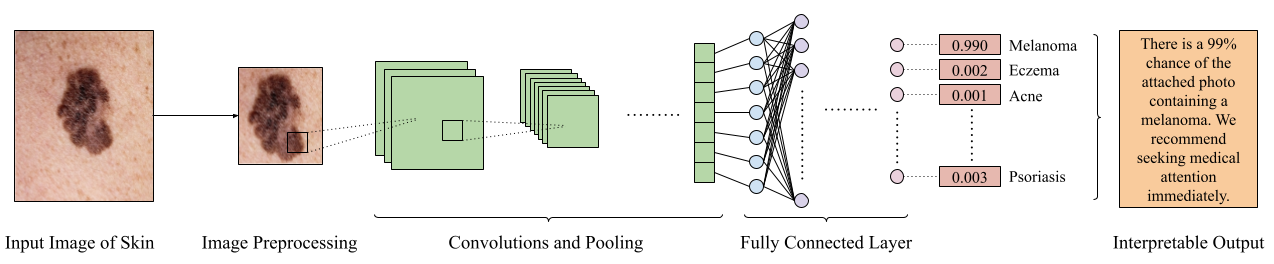
\includegraphics[width=1.0\textwidth]{Figs/project_pipeline.png}
\end{center}
\caption{Overall project pipeline. Dermoscopic, clinical, and patient-taken images of skin conditions are extracted from datasets and preprocessed to resize and remove features. These modified images are passed into a pre-trained CNN to extract image features, which are then inputted into a fully connected classification network, which will output the predicted skin disease and next steps for the patient.}
\end{figure}


\section{Background \& Related Work}
\label{sec:background}

Machine learning models for skin disease detection have been widely studied and are now available to consumers through websites and mobile applications.

\subsection{Deep Convolutional Neural Network to Detect Skin Cancer}

Several studies focus on detecting skin cancers from images. For example, a landmark 2017 study compared the performance of two convolutional neural network (CNN) models—trained on over 120,000 images to distinguish between keratinocyte carcinomas and benign seborrheic keratoses, as well as malignant melanomas and benign nevi—with the diagnostic accuracy of 21 board-certified dermatologists \citep{esteva2017dermatologist}.

Unlike earlier models limited to standardized dermoscopy and histology images, this model was trained to handle dermoscopy and smartphone-quality images, improving usability for everyday users. The model is a deep convolutional neural network, specifically Inception v3, designed by Google for large-scale image recognition. The model achieved higher sensitivity and specificity than the average of the 21 dermatologists.

\begin{figure}[h]
\begin{center}
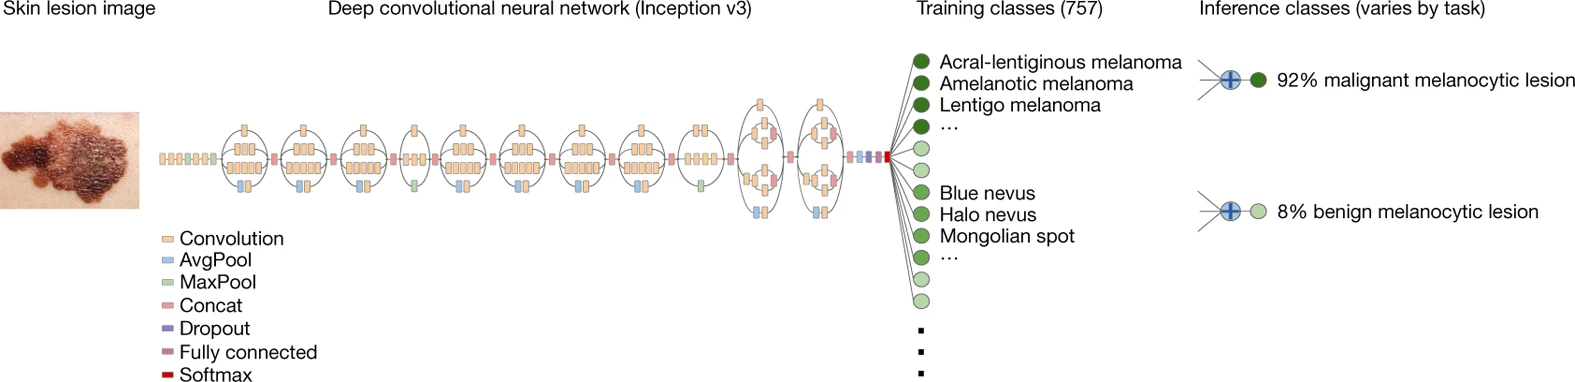
\includegraphics[width=0.9\textwidth]{Figs/inceptionv3.png}
\end{center}
\caption{Google Inception v3 skin cancer classification model architecture \citep{esteva2017dermatologist}.}
\end{figure}

\clearpage

\begin{figure}[h]
\begin{center}
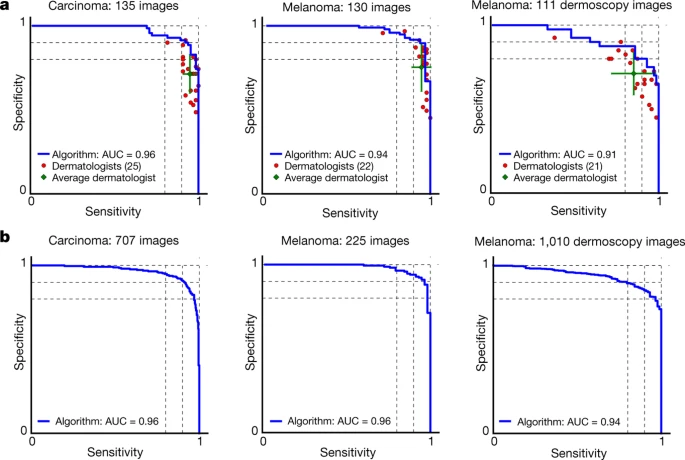
\includegraphics[width=0.9\textwidth]{Figs/auc_roc_inception.png}
\end{center}
\caption{AUC-ROC curve of skin cancer classification performance for Google Inception v3 model \citep{esteva2017dermatologist}.}
\end{figure}

\subsection{Microsoft ResNet for Detecting Skin Conditions}

Another study used the Microsoft ResNet-152 CNN model, trained on 19,398 images, to assess the probability of 12 distinct skin conditions and to differentiate between benign and malignant cases. The model achieved AUC scores ranging from 0.82 to 0.96, comparable to healthcare professionals \citep{han2018classification}.

\subsection{Variations of ResNet Models}

Variations of ResNet have been implemented frequently in studies. For example, a 2025 study uses a self-reliant residual network (SR-ResNet) to identify melanoma \citep{radhika2025self}. It uses Zoutendijk's Method, a nonlinear optimizer that selects optimal step size and direction to stabilize convergence and prevent gradient vanishing and overfitting. The model achieved an accuracy of 94.79\%, precision of 93.09\%, and recall of 96.62\%, outperforming traditional deep learning models \citep{radhika2025self}.

\clearpage

\begin{figure}[h]
\begin{center}
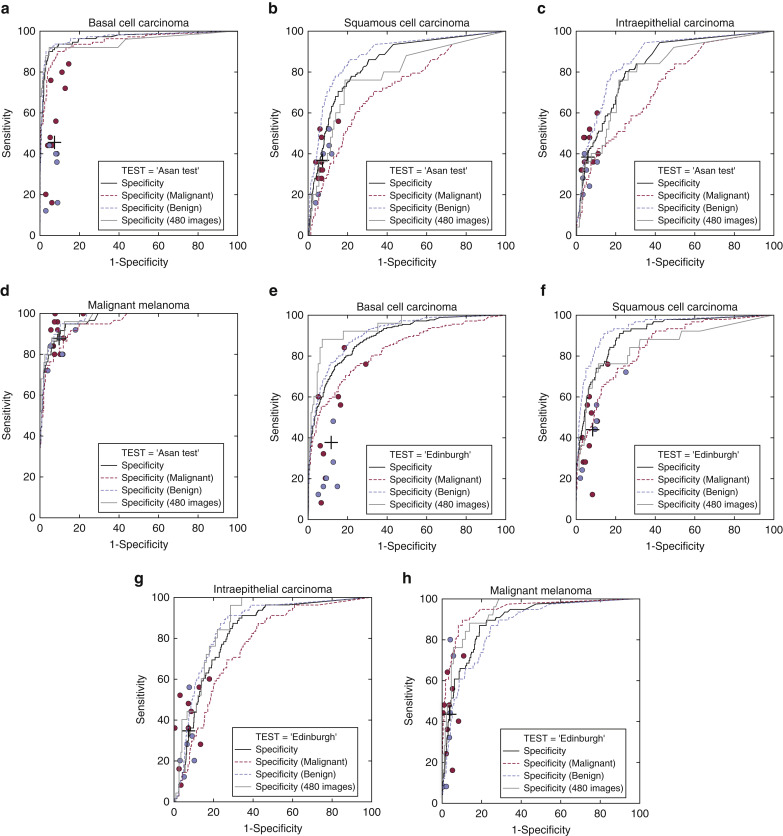
\includegraphics[width=0.9\textwidth]{Figs/auc_roc_sr_resnet.png}
\end{center}
\caption{AUC-ROC curves of classification performance of eight skin cancers for SR-ResNet based model \citep{radhika2025self}.}
\end{figure}

\subsection{Comparisons Between Various Classification Models}

Beyond skin cancer, studies have used models to classify a wider range of skin diseases. For instance, a 2019 study evaluated five different models for classifying three types of skin diseases: Acne, Lichen Planus, and Stevens-Johnson Syndrome/Toxic Epidermal Necrolysis (SJS-TEN), including a Random Forest (RF), Kernel Support Vector Machine (SVM), and CNN \citep{bhadula2019machine}. As before, the CNN was the most successful, achieving high 90s precision and recall scores \citep{bhadula2019machine}. Similarly, a 2025 study classifies both skin lesions and cancers using a convolution self-attention network (CSAN), where convolutional layers extract image features, and a Light Gradient Boosting Machine (LGBM) uses decision trees for final classification \citep{kalpana2025enhancing}. Discrete Mycorrhized Optimization (DMS) optimizes hyperparameters like learning rate and number of trees \citep{kalpana2025enhancing}. Interestingly, in addition to removing noise and resizing images in data preprocessing, the researchers also remove hair to highlight skin. These studies underscore the utility of machine learning, particularly CNNs, in skin disease detection.

\subsection{Websites and Mobile Applications}

Machine learning models that detect skin conditions are readily available on websites and mobile applications. AI Dermatologist, First Derm, and DermascanAI all allow users to upload images of their affected skin at differing prices \citep{aiderm2025,firstderm2025,dermascanai2025}. DermascanAI specifically uses an EfficientNetB0-based network, predicting nine common skin conditions with an accuracy of 87.2\% \citep{vadivelraju2025dermascan}. Smartphones and clinical apps also exist for skin cancer detection. For example, SkinVision detected premalignant and malignant skin lesions with 86.9\% sensitivity and 70.4\% specificity \citep{sangers2022validation}. While accuracy could improve for these models—especially to account for diverse skin tones (see Section \ref{sec:ethics})—these tools help patients self-assess before visiting a doctor and aid clinicians in diagnosis.

\section{Data Processing}
\label{sec:data}

Online databases of common and rare skin conditions involve different imaging techniques. This includes dermoscopic (the most standardised), clinical, and 3D TBP (full body imaging). For the purpose of this project, the dataset must be diverse in the types of imaging technique, which allows the model to generalize. Data augmentation can also be employed to imitate the various imaging techniques. Currently, the objective is to train a model that can classify images taken by medical professionals; however, the objective can be extended to detect images taken by personal cameras, such as the ones in phones.

The following list includes potential datasets that can be used to train the model:

\begin{itemize}
\item \textbf{HAM10000}: Human Against Machine with 10000 Images \citep{ma2018machine}
\begin{itemize}
\item Public dataset released for the purpose of training deep learning models.
\item Images are collected from different populations and modalities, which allows the model to classify people of all skin colors.
\item The dataset is hosted on Kaggle, which allows for direct download in Python \citep{kastle2018skin}
\end{itemize}

\begin{figure}[!h]
\begin{center}
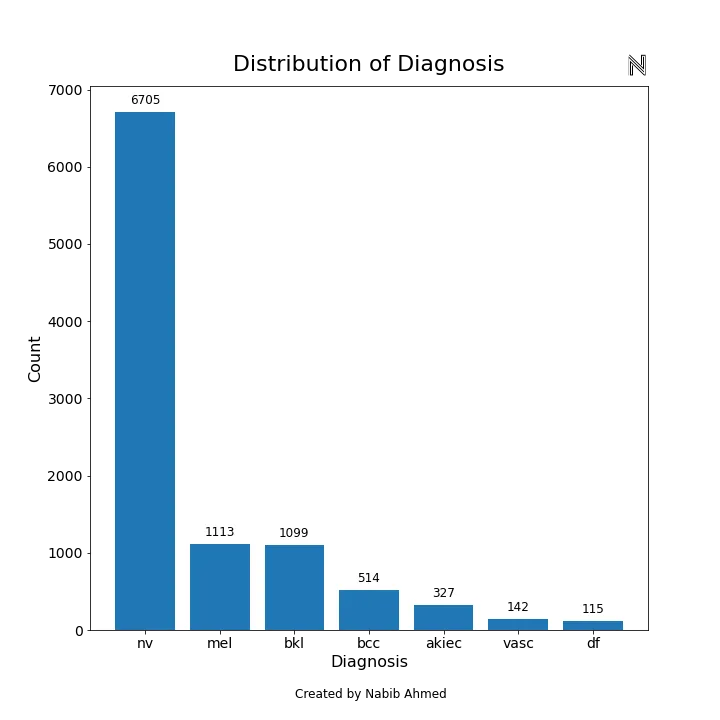
\includegraphics[width=0.5\textwidth]{Figs/ham10000.png}
\end{center}
\caption{Distribution of skin condition classes in HAM10000 dataset \citep{kastle2018skin}}
\end{figure}

\clearpage

\item \textbf{BCN20000} \citep{combalia2019bcn20000}
\begin{itemize}
\item Contains 19,424 dermoscopic images captured under natural (unconstrained) settings in Hospital Clinic Barcelona
\item Provides generalization of lesions that are bigger than the capture range of the dermascope.
\item The dataset is publicly available on the ISIC archives \citep{isic2025bcn}
\end{itemize}

\begin{figure}[!h]
\begin{center}
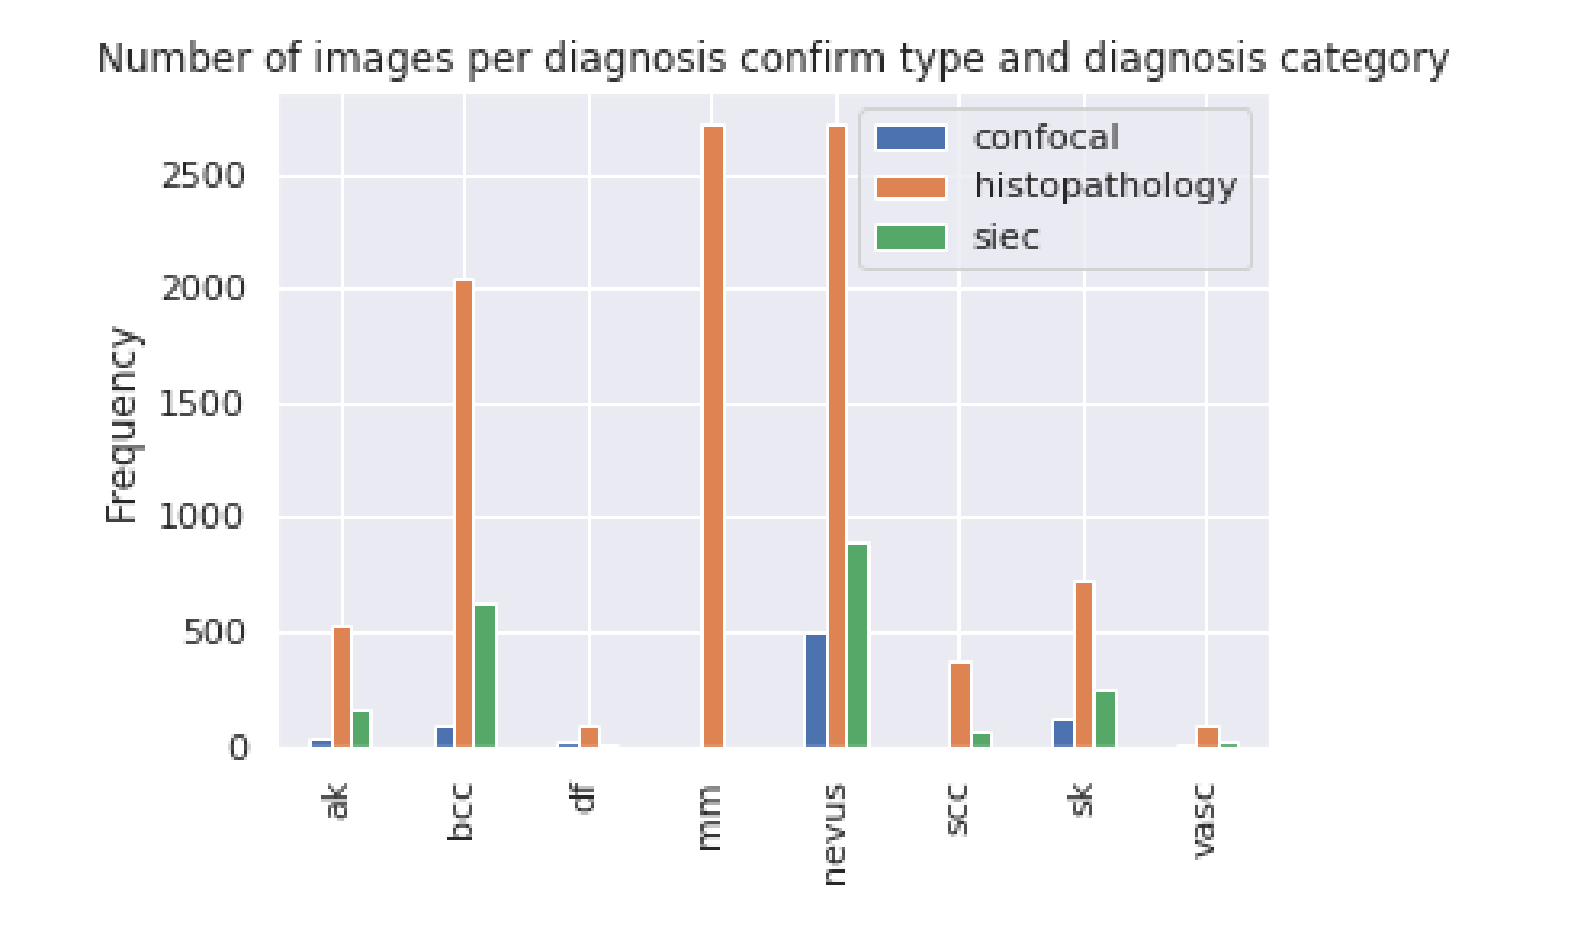
\includegraphics[width=0.7\textwidth]{Figs/bcn20000.png}
\end{center}
\caption{Class distribution and image type in BCN20000 dataset \citep{isic2025bcn}}
\end{figure}

\item \textbf{DERM12345} \citep{yilmaz2024derm12345}
\begin{itemize}
\item Diverse dataset comprising 12,345 dermatoscopic images with 40 subclasses of skin lesions, collected in Turkey.
\item The dataset consists of skin types from the transition zone between Asia and Europe.
\item The dataset access information is available in the article \citep{yilmaz2024derm12345}
\end{itemize}

\item \textbf{ISIC Challenge Datasets} \citep{rotemberg2021patient}
\begin{itemize}
\item The ISIC challenge dataset consists of skin disease images provided to contestants of the ISIC challenge from 2016 to 2020.
\item The dataset is already sorted into training, validation, and testing, which reduces the workload.
\item Citations and sources of the datasets are available on the ISIC website \citep{rotemberg2021patient}.
\end{itemize}
\end{itemize}

If required, additional datasets may be incorporated in the future due to the needs of the project. The datasets will be combined and sorted into training, validation, and testing. This will require all of the images to be adjusted to the same size and format. In addition, the labels will have to be standardized, especially given that the different datasets use different classifications for the diseases. Based on the information provided from the background, the standardized label approach will be image segmentation, where a point or polygonal mask is applied over the lesion (region of interest/disease). The color of the mask will determine the class/disease.

As mentioned before, data augmentation will be used to increase training data and help the model to generalize. Techniques such as brightening/dimming, cropping, zooming in/out, distortion, and gaussian noise will be used to imitate the different imaging devices people and clinics may have access to.

\section{Architecture}

The model architecture will be a Convolutional Neural Network (CNN) with multiple convolutional layers. A CNN can extract spatial features, such as edges, textures, and patterns, using learnable filters, making them ideal for image classification tasks like skin disease detection. Due to computational and time constraints, transfer learning is employed with the pre-trained EfficientNet-B3 or ResNet as the feature extractor, making only the classifier training necessary.

The custom classifier that follows the pre-trained network includes a global average pooling layer to reduce feature dimensionality, multiple fully connected layers using ReLU activation functions, dropout layers to prevent overfitting, and a final output layer with softmax or sigmoid activation depending on the desired output.

The pre-trained backbone will be frozen to train the classifier on the features extracted from the skin images. Once the classifier stabilizes, selected layers of the backbone may be unfrozen for fine-tuning with a reduced learning rate. Cross-entropy loss and Adam will be used as the loss function and optimizer.

\section{Baseline Model}

A good baseline model to use for comparison is a model that utilizes k-nearest neighbour (KNN) or support vector machine (SVM). Numerous skin disease classifiers have been made using these algorithms, and many of them have achieved strong results with accuracies as high as 98\% \citep{sumithra2015segmentation,hatem2022skin,bakheet2017svm,das2013svm}. However, these models typically use highly pre-processed images with a small dataset (typically less than 1000 samples). Moreover, the datasets used do not contain images of healthy skin, completely eliminating the possibility of type 1 (false positive) and type 2 (false negative) errors.

These types of models can be replicated using an implementation of KNN or SVM with the expected classifications and feeding in the dataset. Given that the dataset being used is a combination of various datasets whose images may not be ideally processed, the baseline model is expected to not perform as well. This provides a good opportunity to test if a CNN-based machine learning model would be able to perform better in a more realistic setting.

\section{Ethical Considerations}
\label{sec:ethics}

Machine learning models for skin disease detection raise ethical concerns in both data collection and model use.

Training and validating these models requires labelled images of skin. Datasets that contain private healthcare information like skin images must adhere to patient privacy standards, including patient consent and research ethics board approval. For instance, DermNet, a leading organization for dermatology, requires images not to be identifiable (i.e. no face) and evidence of patient consent before addition to their library \citep{dermnet2025clinical}.

Additionally, existing datasets contain a disproportionately large number of images representing lighter skin tones compared to darker skin tones. This imbalance results from lower skin cancer rates in darker-skinned individuals and unequal access to healthcare \citep{alipour2024skin}. It impairs model performance for patients with darker skin, potentially reinforcing pre-existing healthcare disparities across racial and ethnic groups. To mitigate this issue, some skin datasets, such as SkinCon, include Fitzpatrick skin type labels while others like DDI include equal numbers of each skin type \citep{daneshjou2022skincon,daneshjou2022disparities}.

Beyond data collection concerns, a skin disease detection model also risks patients misinterpreting model outputs. For example, if the model incorrectly classifies a mild condition as severe, they may face unnecessary anxiety. Conversely, if the model fails to detect a serious condition, patients may delay or avoid medical advice and treatment, worsening their skin condition. Patients must understand that the model is only an aid—not a replacement for proper diagnosis. To mitigate these risks, models should prioritize high recall to minimize missed detections of serious conditions.

\section{Project Plan}

The team's main source of communication will be through a group chat, where discussions happen on a daily basis. All team members live within the GTA, which allows for in-person meetings.

Moving forward, the team will hold weekly meetings online/in-person to discuss project progress and next steps. At the meeting, each team member will be expected to report the tasks they have completed or the progress they have made to accomplish said task. In addition, new tasks may be assigned to team members depending on their availability and progress. All tasks, assignees, and progress will be tracked using monday.com, which is a web-based app for work management.

Figure 6 provides a rough summary of the tasks, assignees, and deadlines outlining the project. Since certain tasks may have the same deadline, priority will be assigned to each task so team members can prioritize more urgent tasks.

\begin{figure}[h]
\begin{center}
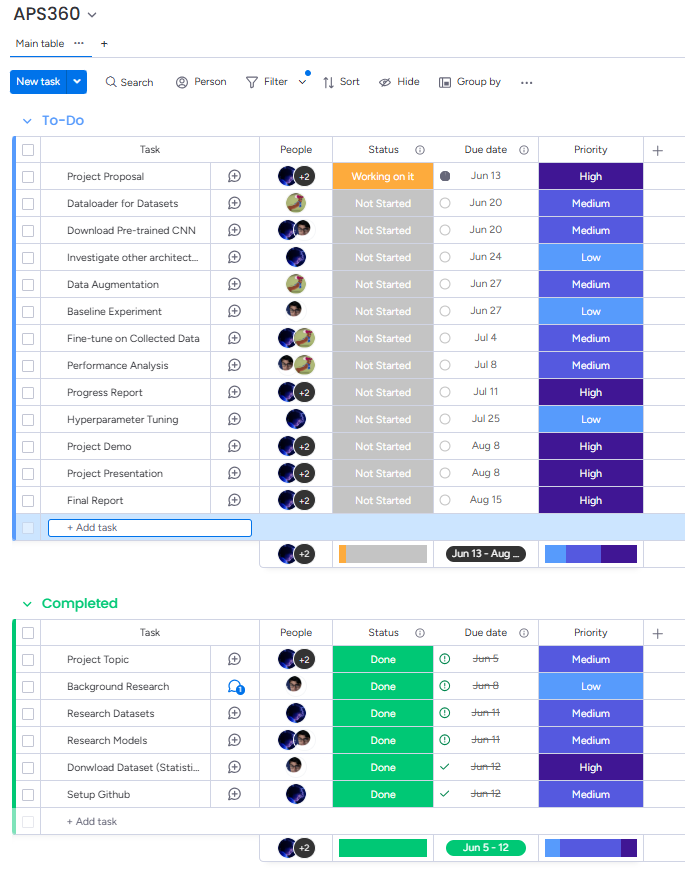
\includegraphics[width=0.7\textwidth]{Figs/project_task_outline.png}
\end{center}
\caption{Project task outline created using monday.com}
\end{figure}

The team will collaborate in their work on Github, while training may be done on Google Colab due to the lack of GPUs. Project files, such as Python scripts and Jupyter notebooks will be stored in the team's public Github repository. New branches will be created for specific tasks to avoid overwriting existing code. Once a task is complete, developers may open pull requests, then merge the completed code into master after code reviews.

\clearpage
\section{Risk Register}

Potential risks for the project are listed below.

\subsection{Team Members Dropping The Course}

After a team discussion, we determined that the likelihood of a team member dropping the course is small, however, non-zero. In the case that a team member does drop the course, it is important that we have properly documented each stage of the project and explicitly parceled out tasks. In this way, the remaining team members can easily take over the responsibility of the team member who dropped the course. The general outline for this has been given in the Project Plan section and we will continue in a similar manner on a shared Google Doc and in our team Discord as the project progresses. Even without the risk of a team member dropping, proper documentation and task assignment is still of paramount importance to working efficiently as a team.

\subsection{Busy Work Schedules}

Each of our team members have other commitments, for example, we are all involved in summer research programs. This can lead to conflicts with meeting times and work schedules. This issue is very likely to arise, in fact, in the process of working on this project proposal it has already become apparent. When encountering this issue, it is important that we maintain effective communication and work together around each other's schedules. As a team, we have already implemented this strategy and seen success from it. Team members communicated their availability for working on the project proposal and we coordinated tasks accordingly, allowing us to make steady progress despite our conflicting commitments.

\subsection{Unexpected Training Time}

A potential risk we foresee is that training time may be longer than expected, which could result in missing important deadlines. This is a fairly likely scenario, given that training times are highly variable. However, this risk can be effectively mitigated with proactive planning. To address this, we will train a baseline model early in the process to establish a rough estimate of how long model training typically takes in our environment. This initial benchmark will help us better schedule future training sessions and avoid last-minute surprises. Additionally, we plan to schedule final model training at least one full day in advance of any deadlines to allow for grace time in case of unexpected delays or errors. This buffer will give us room to troubleshoot issues without compromising our timeline.

\subsection{Poor Model Performance}

Due to the variety of skin diseases in our datasets, we find it fairly likely that our model fails to classify images with an acceptable accuracy (85+\%) and recall, which is particularly important for medical diagnosis tools which should not miss positive cases. To minimize this risk, we will train the model with a combination of multiple datasets including the datasets mentioned in Section \ref{sec:data}, use transfer learning to prevent overfitting, remove hair from images in preprocessing, and add extra noise to data. If the model has difficulty predicting minority classes, we can increase the weighting of minority classes in the training or generate artificial examples. If these steps are still insufficient, we can limit our model to predict skin conditions with greater data availability like eczema, acne, and melanoma.

\section{Link to Colab/GitHub}

Github Repository containing all source code is publicly available at \url{https://github.com/jakkiiri/APS360-Project}

\label{last_page}

\clearpage
\bibliography{APS360_ref}
\bibliographystyle{iclr2022_conference}

\end{document}
